\chapter{Lösungsansatz}

Im Folgenden werden unsere Herangehensweisen an das Problem beschrieben. Wir untersuchen den Übergang zwischen einem schläfrigen Zustand, ohne kognitive Beanspruchung, und einem wachen Zustand, in dem Aufgaben von der Testperson übernommen werden können. Hierzu bietet sich aus zeitlichen Gründen eine Untersuchung mittels virtueller Realität an. Wir betrachten außerdem eine Reihe von Aufgaben, die in VR durchgeführt werden und einen Bezug auf reale Situationen im Kontext Autofahren aufweisen.

\section{Idee}

Wir möchten die Teilnehmer der Studie dazu bringen einen Zustand zu erreichen in dem das fehlerfreie Erledigen von Aufgaben eine gewisse geistige Anstrengung aufweist. Dies ist vergleichbar damit, dass im Straßenverkehr das autonome Fahren dem Fahrer erlaubt seine Aufmerksamkeit von der Straße zu nehmen, seinen Sitz zu kippen und die Augen zu schließen. Sollte der Fahrer daraufhin von seinem Fahrzeug aufgefordert werden in eine Situation einzugreifen und eine Entscheidung zu treffen, wie Beispielsweise einen schwierigen Abschnitt der Strecke selbst zu Fahren, oder eine Entscheidung zu treffen, muss das Fahrzeug den Fahrer aufwecken und informieren. In diesem Zustand könnten Informationen nur schwer aufgenommen werden und eine Aufgabe, die in diesem Zeitraum gestellt wird könnte so mit geringerem Erfolg erledigt werden, als wenn der Fahrer voll aufnahmefähig ist.

\todoAll{Dieses Paper könnte interessant sein, warum Entscheidungen von Menschen getroffen werden sollten... \cite{awad2018moral}. Es geht prinzipiell nur darum diese Entscheidung von einem neuronalen Netz übernehmen zu lassen und ich habe bis jetzt nicht rein geschaut, aber vielleicht stehen ja auch noch interessante Sachen drin. Für die Interessierten: 'Moral Machine' bei google eingeben -tl}

Wir untersuchen in dieser Arbeit nicht die Auswirkungen des Schlafens, oder des Mangels an Schlaf auf das Gehirn, sondern viel mehr die Überführung von einem trägen oder schläfrigen Zustand in einen Wachen. 

Um eine möglichst kontrollierbare Testumgebung mit vergleichbaren Ergebnissen zu haben nutzen wir VR in einem separaten Raum der Universität Ulm. Hier werden die Teilnehmer gebeten mit dem VR-HMD in einer initialen Phase zu entspannen. Das Ziel ist es die beschriebene Situation der geringeren Aufnahmefähigkeit und Schläfrigkeit zu erzeugen, wie er auch nach dem Schlafen auftreten kann. 

Im Anschluss an die Ruhephase werden die Nutzer auf unterschiedliche Arten "`aufgeweckt' und ihnen werden drei Aufgaben gestellt. Die von uns untersuchten Arten des Weckens sind Licht und Ton. Wobei die Einstellung des Lichts noch in zwei weitere Gruppen unterteilt ist. Für Gruppe eins wird das licht innerhalb von 5 Sekunden von 0\% Intensität auf 100\% erhöht, bei Gruppe zwei geschieht dies Über einen Zeitraum von 20 Sekunden. 
Allen drei Gruppen werden im Anschluss die Aufgaben iterativ präsentiert.

Auf dieser Grundlage formulieren und untersuchen wir die folgenden Hypothese auf:

\begin{hyp}[H\ref{hyp:lichtSchneller}]\label{hyp:lichtSchneller}
	Menschen, die mit Licht geweckt werden, können sich in kürzerer Zeit auf eine gestellte Aufgabe einstellen, als Menschen, die mit Ton geweckt werden.
\end{hyp}

\begin{hyp}[H\ref{hyp:lichtErfolgreicher}]\label{hyp:lichtErfolgreicher}
	Menschen die mit Licht geweckt werden, können eine gestellte Aufgabe mit weniger Fehlern erledigen, als Menschen, die mit Ton geweckt werden.
\end{hyp}

\begin{hyp}[H\ref{hyp:langKurzSchneller}]\label{hyp:langKurzSchneller}
	Menschen die langsam geweckt werden können sich in kürzerer Zeit auf eine gestellte Aufgabe einstellen, als Menschen, die abrupt aus dem Schlaf gerissen werden.
\end{hyp}

und 

\begin{hyp}[H\ref{hyp:langKurzErfolgreicher}]\label{hyp:langKurzErfolgreicher}
	Menschen die langsam geweckt werden können eine gestellte Aufgabe mit weniger Fehlern erledigen, als Menschen, die abrupt aus dem Schlaf gerissen werden.
\end{hyp}

\subsection{Aufwachen}
Probanden können auf unterschiedliche Arten aufgeweckt werden~\cite{jewett1999time, ferrara2000sleep}
\begin{itemize}
	\item \textbf{Töne}
	\item \textbf{Licht}
\end{itemize}
\todoAll{Beschreiben... und noch auf verwandte Forschung eingehen}
\todoLuc{Warum haben wir gewisse Paramter ausgesucht}

\section{Testaufbau}
Sitzend werden Probanden erst in einen entspannten Zustand versetzt. In diesem verweilen sie möglichst ohne Ablenkung, bis sich eine Gelassenheit oder Trägheit einstellt. Diese kann von entspanntem Sitzen bis hin zum Schlaf führen, eine genaue Zeitspanne hierfür kann zwischen Probanden variieren und muss in Tests bestimmt werden.

Nachfolgend wird der Teilnehmer aus diesem Zustand geleitet und mit einer Aufgabe konfrontiert. Während der Erledigung dieser werden unterschiedliche Parameter aufgezeichnet und später ausgewertet. Die erfassten Parameter sind die folgenden:

\begin{itemize}
	\item Zeit in der eine Aufgabe erledigt wird
	\item Fehlerrate bei der Erledigung der Aufgabe
	\item Blickrichtung
\end{itemize}\todoTob{Redundant mit der Implementierung... wo soll das am ehesten hin?}

Die erste Studie umfasst ungefähr 30 Minuten, hierfür werden die Teilnehmer mit fünf Euro entlohnt. Der Ablauf der Studie Umfasst folgende Punkte:

\begin{enumerate}
	\item \textbf{5 Minuten} Vorbereitung und Einführung in den Studienablauf inklusive der Bedienung der VR-Umgebung
	\item \textbf{15 Minuten} Beruhigungsphase bis hin zum Schlafen
	\item \textbf{3-5 Minuten} Aufgaben lösen
	\item \textbf{5 Minuten} Fragebögen beantworten
\end{enumerate}

Die Fragebögen, die wir heranziehen sind zum einen der NASA TLX und ... \todoAll{Raus damit? Oder beschreiben}

Es handelt sich um eine between subject Studie. Im ersten Durchlauf erfassen wir die genannten Parameter unter der Betrachtung der Zeit in der die virtuelle Umgebung erhellt wird. Die genauen Zeiten werden in einer Testphase während des Implementierens eingegrenzt.

Zudem werden die Probanden entweder mit Ton oder durch einen Lichtreiz "`geweckt"'. Auch dieser Parameter wird in einer Testphase experimentell angenähert.

\subsection{Aufgaben}
Die Aufgaben sollen die Aufnahme- und Leistungsfähigkeit der Studienteilnehmer überprüfen. Hierzu wurden Aufgaben gewählt für dessen Erledigung keinerlei Erfahrung mit Virtual-Reality Geräten vorausgesetzt wird. Die Übungen sind verständlich und auch ohne Spielerfahrung bewältigbar.
Insgesamt werden dem Probanden drei Aufgaben gestellt. 
%Jede einzelne von ihnen lässt sich durch wiederholtes, einfaches Zielen mit dem Controller und %anschließendem Betätigen einer Taste bewältigen.
 
% Um die Spiele zu entwickeln können aber auch Toolboxes und Frameworks herangezogen werden, so zum Beispiel auch~\cite{devisch2018mini}.
% Die validierung der Spiele gestaltet sich als schwierig, oder findet jemand noch Quellen? Kann man auch sagen, da es sich nicht um spiele handelt, gestaltet man Aufgaben, die (abstrakt) nahe an eine reale Tätigkeit herankommen? Oder kann man argumentieren, dass hier die gewählten Aufgaben einer realen Tätigkeit entsprechen?

\subsubsection{Zahlenfolge} 
Verteilt über das Blickfeld des Probanden werden Zahlen angezeigt. Die Abstände zwischen den Zahlen sind nicht gleichverteilt und werden idealerweise so gewählt, dass eine Verwechslungsgefahr besteht. Aufsteigend sollen die Zahlen selektiert und so geordnet werden. Diese Aufgabe soll das schnelle Wahrnehmen bekannter Elemente (in diesem Fall das Wahrnehmen von Zahlen) und die Fähigkeit des numerischen Sortierens Prüfen. 
%Evtl noch ein bisschen ausschmücken.
(123 $\rightarrow$ 324 $\rightarrow$ 823 $\rightarrow$ 1237 ...)

\begin{figure}
	\centering
	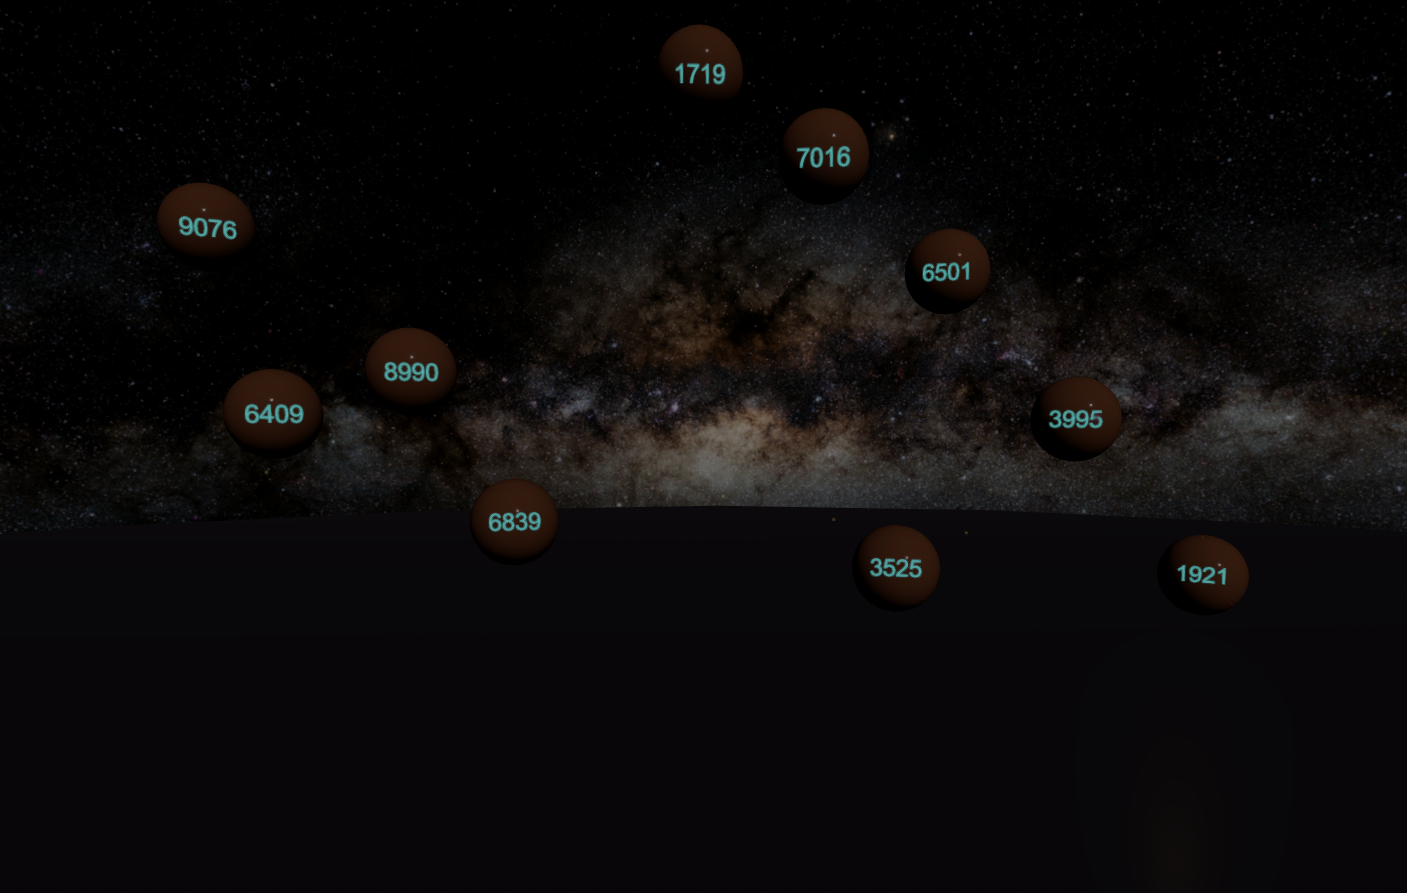
\includegraphics[width=0.8\textwidth]{./images/ordering.png}
	\caption{Erste Aufgabe der Studie. Der Text auf den Kugeln soll in aufsteigender Reihenfolge sortiert ausgewählt werden.}
	\label{fig:ordeing}
\end{figure}

\subsubsection{Stroop-Effekt} 
Im Mittelpunkt des Blickfeldes wird eine ausgeschriebene Farbe angezeigt. Die Textfarbe des Worts muss nicht zwangsläufig die der ausgeschriebenen Farbe sein. Der Proband soll als Eingabe die Textfarbe auswählen indem er mit dem Controller auf einem Interface die richtige Auswahl trifft. Beispiel kann in Figure~\ref{fig:matching} gesehen werden. Diese Aufgabe dient dem Testen von ungewohnten Aufgaben, welche dem Anwender in der Regel nicht vertraut sind und auf welche sich der Proband in kürzester Zeit einstellen muss.

\begin{figure}
	\centering
	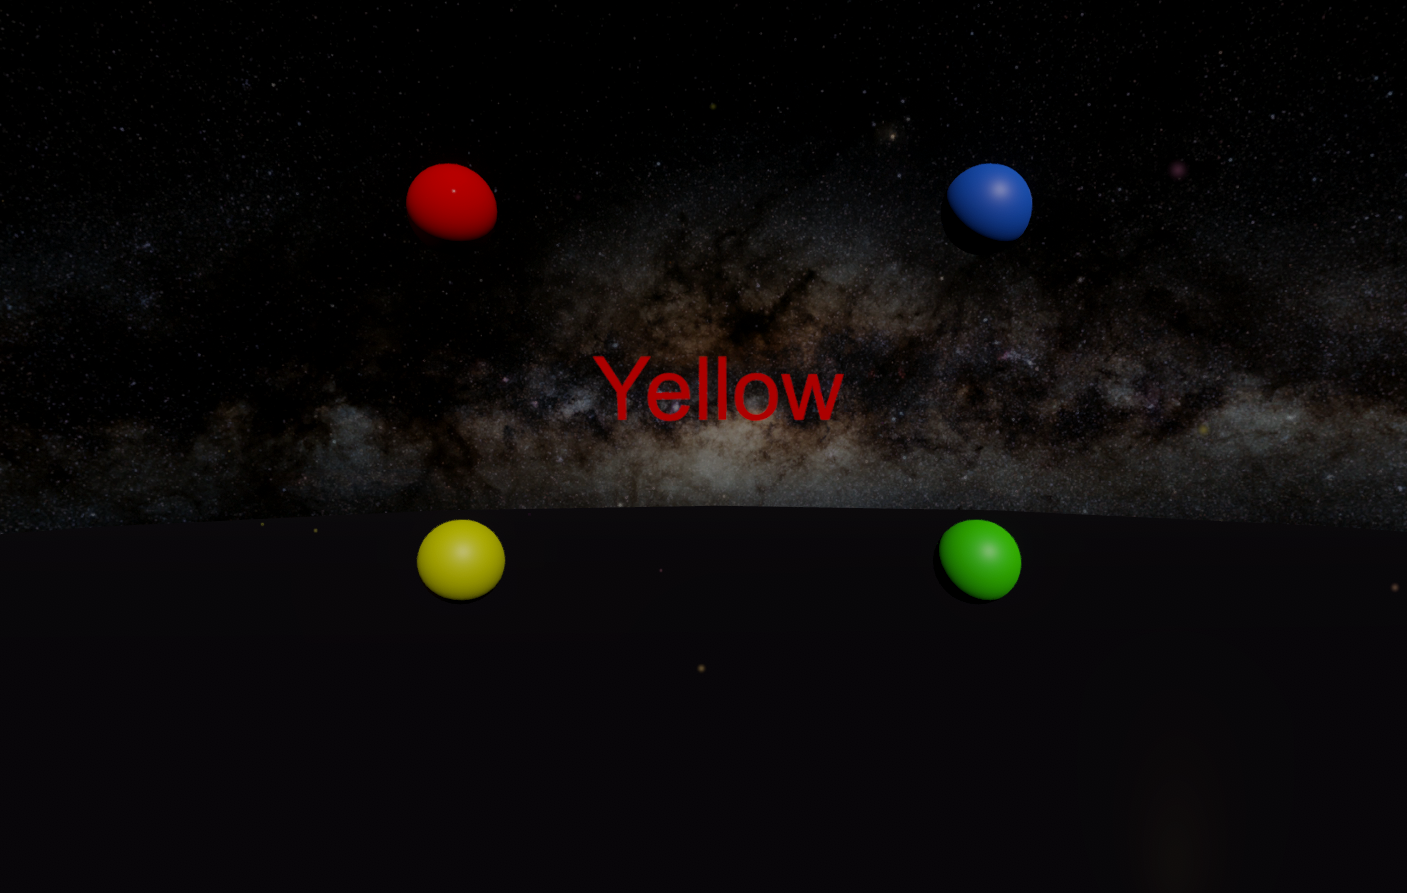
\includegraphics[width=0.8\textwidth]{./images/matching.png}
	\caption{Zweite Aufgabe. Teilnehmer der Studie sollen die Farbe, welche in Textform im Sichtbaren Bereich steht auswählen. Es soll nicht die gleiche Farbe ausgewählt werden.}
	\label{fig:matching}
\end{figure}

\subsubsection{Boxen zählen} 
In isometrischer Ansicht werden eine Vielzahl von Boxen innerhalb der virtuellen Umgebung angezeigt. Die Boxen stehen aufeinander und verdecken zum Teil den Blick auf andere Boxen. Es soll durch die Schlussfolgerung, dass diese, so wie in der realen Welt, nicht in der Luft schweben können, die Anzahl der Boxen gezählt und ausgewählt werden. Diese Aufgabe konzentriert sich auf das räumliche Wahrnehmen und Vorstellungsvermögen des Anwenders.

\begin{figure}
	\centering
	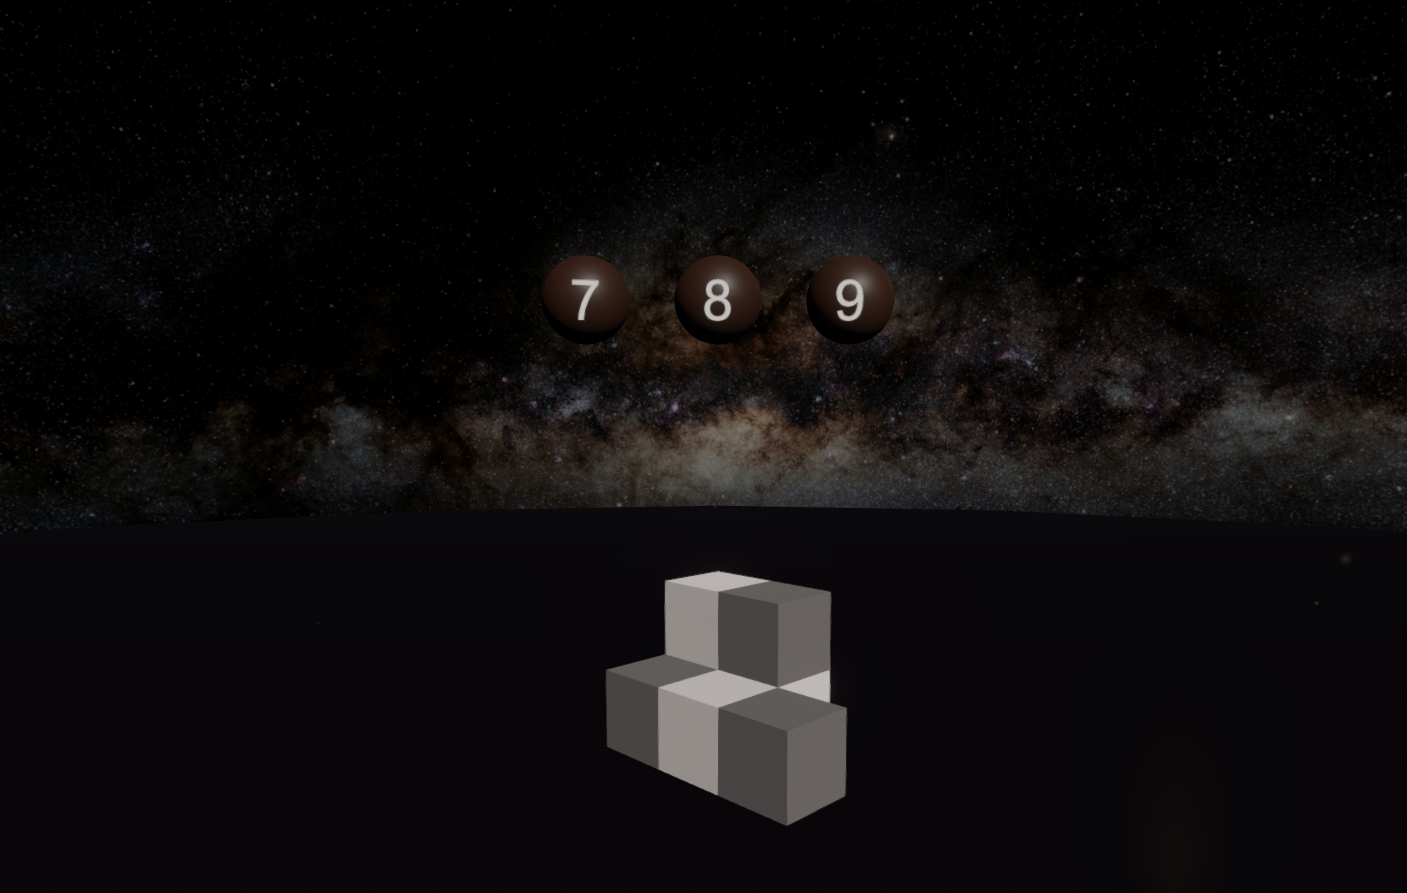
\includegraphics[width=0.8\textwidth]{./images/counting.png}
	\caption{Dritte Aufgabe in der virtuellen Umgebung. Die Teilnehmer sollen die Anzahl der Boxen zählen. Boxen verdecken die Sicht auf andere Boxen. Sie können nicht in der Luft schweben.}
	\label{fig:counting}
\end{figure}

\subsection{Studienumgebung}
\todoSab{Hier bitte die Räumlichkeiten kurz beschreiben, also Raum, Licht, Störfaktoren etc.}

%  ===== THIS IS INTENTIONALLY LEFT HERE AS REFERENCE FOR SUBFIGURES (copy&paste)
% \begin{figure}
% 	% \centering
% 	\begin{subfigure}{0.4\textwidth}
% 		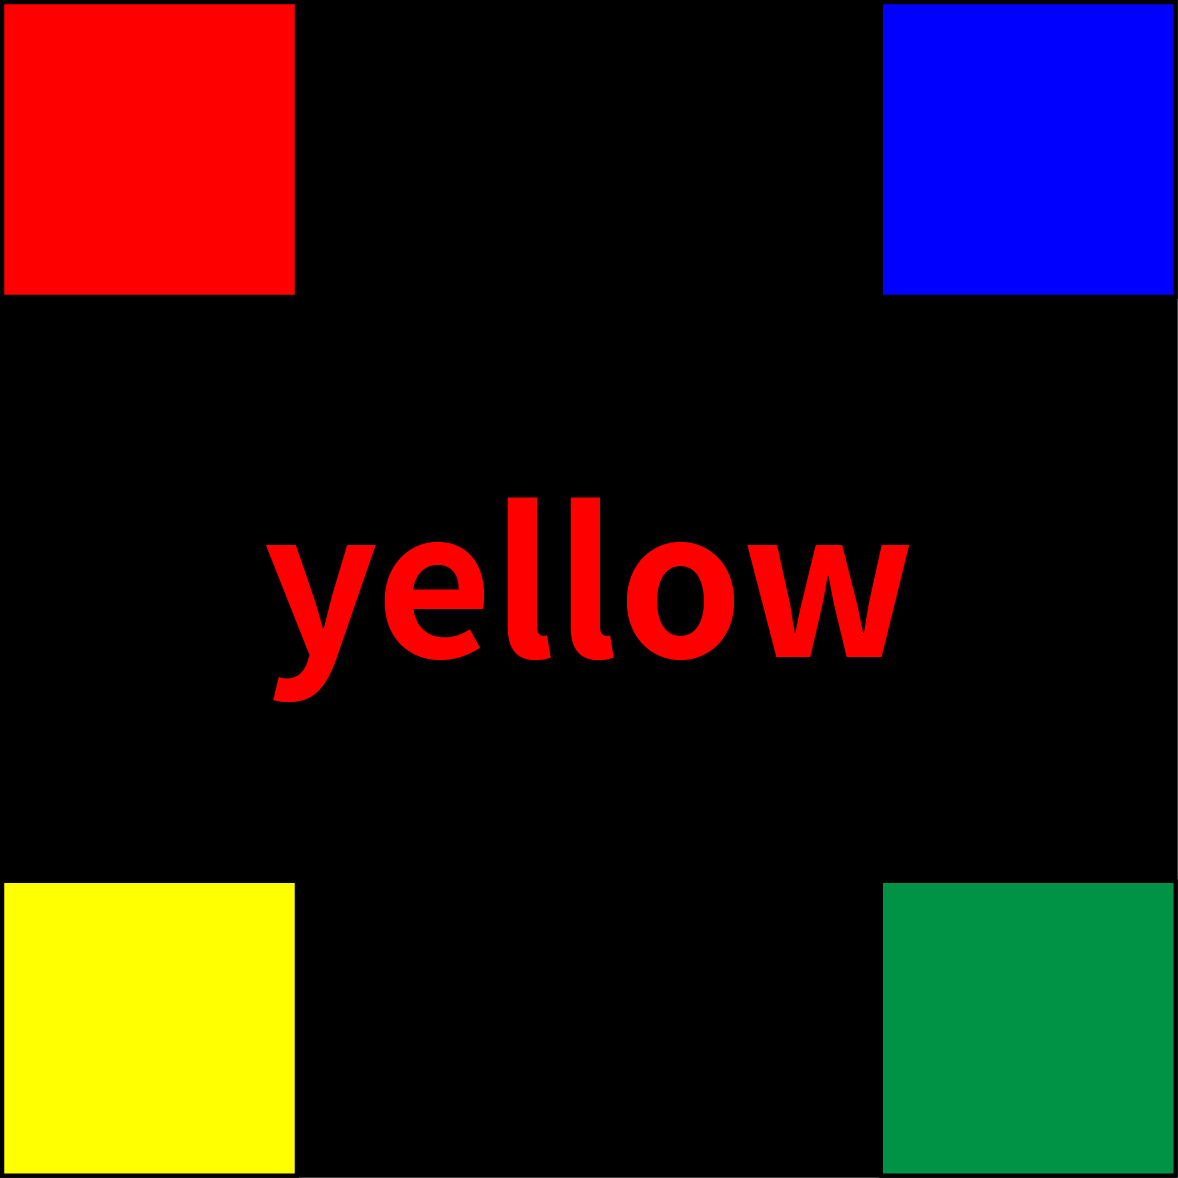
\includegraphics[width=\textwidth]{./images/Reversed_stroop_test.jpg}
% 		\caption{Stroop Test, ElvisLin CC BY-SA 4.0. \url{https://commons.wikimedia.org/wiki/File:Reversed_stroop_test.jpg}} % subcaption
% 		\label{fig:stroop_test}
% 	\end{subfigure}%
% 	\hfill
% 	\begin{subfigure}{0.5\textwidth}
% 		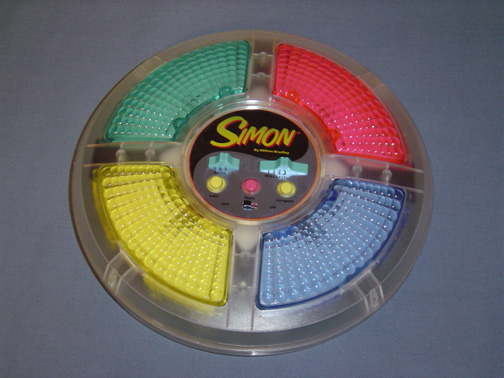
\includegraphics[width=\textwidth]{./images/Simon_game.jpg}
% 		\caption{Senso / Simon, Larry D. Moore CC BY-SA 3.0. \url{https://commons.wikimedia.org/wiki/File:Simon_game.jpg}} % subcaption
% 		\label{fig:simon}
% 	\end{subfigure}
% 	\caption{Beispiele für die Spiele mit denen die Teilnehmer konfrontiert werden.} % caption for whole figure
% \end{figure}
